%% LyX 2.4.4 created this file.  For more info, see https://www.lyx.org/.
%% Do not edit unless you really know what you are doing.
\documentclass[english]{article}
\usepackage[T1]{fontenc}
\usepackage[latin9]{inputenc}
\usepackage{units}
\usepackage{enumitem}
\usepackage{amsmath}
\usepackage{amsthm}
\usepackage{cancel}
\usepackage{geometry}
\geometry{verbose,tmargin=1in,bmargin=1in,lmargin=1in,rmargin=1in}

\makeatletter
%%%%%%%%%%%%%%%%%%%%%%%%%%%%%% Textclass specific LaTeX commands.
\numberwithin{equation}{section}
\numberwithin{figure}{section}
\newlength{\lyxlabelwidth}      % auxiliary length 

%%%%%%%%%%%%%%%%%%%%%%%%%%%%%% User specified LaTeX commands.
\usepackage{fancyhdr}
\usepackage{lastpage}
\pagestyle{fancy}
\usepackage{enumitem}
\usepackage{ifthen}
%sets math fonts to be more readable
\everymath=\expandafter{\the\everymath\displaystyle}
%\DeclareMathSizes{10}{10}{10}{10}
\usepackage{multicol}

\usepackage{tikz}
\usetikzlibrary{plotmarks}
\usepackage{pgfplots}
\pgfplotsset{compat=newest}

\usepackage{calc}
\usepackage[nomessages]{fp}

\usepackage{advdate}    % Advancing/saving dates
\usepackage{datetime}   % Dates formatting
\usepackage{datenumber} % Counters for dates
% Added by lyx2lyx
\setlength{\parskip}{\smallskipamount}
\setlength{\parindent}{0pt}

\makeatother

\usepackage{babel}
\begin{document}
\renewcommand{\author}{Dr.\,James Ashe}

\newcommand{\classNum}{131}

\newcommand{\classSec}{B}

\newcommand{\nameType}{Name:}

\newcommand{\examType}{Exam 3 (make-up)}

\renewcommand{\date}{\formatdate{1}{11}{2013}}

%%First page's header%%%%%%%%%%%%%%%%%%%%%%
\fancypagestyle{firststyle} %%header settings for first pagr
{
	\fancyhead[L]{MTH \classNum{}(\classSec{}) \author{}\\
	\textbf{\examType{}} \date{}}
	\fancyhead[C]{\textbf{\nameType}}
	\setlength{\headsep}{14pt}
}
%%%%%%%%%%%%%%%%%%%%%%%%%%%%%%%%%%%%%%%%%%

%%Next page's header%%%%%%%%%%%%%%%%%%%%%%%
\setlist{nolistsep}
\lhead{MTH \classNum{}(\classSec{})} 
\chead{\textbf{\nameType}} 
\cfoot{\thepage{}~of~\pageref{LastPage}} 
\setlength{\headsep}{5pt} 
%%%%%%%%%%%%%%%%%%%%%%%%%%%%%%%%%%%%%%%%%%%

%%Various settings; see the preamble for other settings%%%%%
%\setenumerate[0]{leftmargin=12pt,itemindent=0pt,labelwidth=0pt}
%\setlist[enumerate]{topsep=0pt,itemsep=1pt,partopsep=1ex,parsep=1ex}
\renewcommand{\labelenumi}{\textbf{\arabic{enumi}.}}
\renewcommand{\labelenumii}{\textbf{\alph{enumii}.}}
\thispagestyle{firststyle}
%%%%%%%%%%%%%%%%%%%%%%%%%%%%%%%%%%%%%%%%%%
\newcommand{\xmax}{10}
\newcommand{\xmin}{-10}
\newcommand{\xstep}{0} %must be xmin+n
\newcommand{\ymax}{10}
\newcommand{\ymin}{-10}
\newcommand{\ystep}{0} %must be ymin+n

\newcommand{\xspace}{\vspace{1cm}}
\gdef\listCount{1}

\textbf{Use the function }$f(x)=(x-2)^{2}-6$\textbf{ to answer problems
\ref{enu:.f(x)}--\ref{f(X) last}.}

\begin{multicols}{2}
\begin{enumerate}[resume]
\item \label{enu:.f(x)}Find the coordinates of the vertex for the parabola
defined by $f(x)$.\xspace\xspace
\item Find the axis of symmetry of the parabola defined by $f(x)$.\xspace
\item Find the range of $f(x)$.\xspace
\item \label{f(X) last}Graph $f(x)$ clearly showing the vertex and \emph{y-}intercept.\xspace\columnbreak
\item []\vspace{0cm}\renewcommand{\xmax}{10} 
\renewcommand{\xstep}{5}
\renewcommand{\ymax}{\xmax} 
\renewcommand{\ystep}{5}
%%%%%%%
\begin{tikzpicture} 
	\begin{axis}[
		axis x line=middle, axis y line=middle,     		
		xtick={-\xmax,-\xstep,...,\xmax},
		ytick={-\ymax,-\ystep,...,\ymax},
		minor x tick num={4},
		minor y tick num={4},
		grid=both,
		xlabel={$$},     
		ylabel={$$},
		xmin=-\xmax.25,xmax=\xmax.25,
		ymin=-\ymax.25,ymax=\ymax.25,     		width=6cm,     		height=6cm] 		
%\addplot[red,very thick,mark=noner,smooth,domain=\xmin:\xmax]{-(x-2)^2+6}; 
	\end{axis}
\end{tikzpicture}\gdef\listCount{5}
\end{enumerate}
\end{multicols}\vfill

\textbf{Use the function }$g(x)=-x^{2}+4x+4$\textbf{ to answer problems
\textbf{\listCount}--\ref{f(X) last-1}.}

\begin{multicols}{2}
\begin{enumerate}[resume]
\item [\textbf{\listCount.}] \setcounter{enumi}{\listCount}Find the coordinates
of the vertex for the parabola defined by $g(x)$.\xspace\xspace
\item Find the minimum of $g(x)$.\xspace
\item Find the domain of $g(x)$.\xspace
\item \label{f(X) last-1}Graph $g(x)$ clearly showing the vertex and \emph{y-}intercept.\xspace\columnbreak
\item []\vspace{0cm}\renewcommand{\xmax}{10} 
\renewcommand{\xstep}{5}
\renewcommand{\ymax}{\xmax} 
\renewcommand{\ystep}{5}
%%%%%%%
\begin{tikzpicture} 
	\begin{axis}[
		axis x line=middle, axis y line=middle,     		
		xtick={-\xmax,-\xstep,...,\xmax},
		ytick={-\ymax,-\ystep,...,\ymax},
		minor x tick num={4},
		minor y tick num={4},
		grid=both,
		xlabel={$$},     
		ylabel={$$},
		xmin=-\xmax.25,xmax=\xmax.25,
		ymin=-\ymax.25,ymax=\ymax.25,     		width=6cm,     		height=6cm] 		
%\addplot[red,very thick,mark=noner,smooth,domain=\xmin:\xmax]{4+x^2+4*x}; 
	\end{axis}
\end{tikzpicture}\gdef\listCount{9}
\end{enumerate}
\end{multicols}

\newcommand{\picW}{4.5cm} \newcommand{\picH}{\picW}

\vfill\textbf{The graph of the function is given. Determine the function's
equation.}
\begin{enumerate}[resume]
\item [\textbf{\listCount.}] \setcounter{enumi}{\listCount}\hspace{0cm}

\begin{enumerate}[resume]
\item []\renewcommand{\xmax}{10} \renewcommand{\xstep}{5}
\renewcommand{\ymax}{\xmax} \renewcommand{\ystep}{5}
%%%%%%%
\begin{tikzpicture} 
	\begin{axis}[
		axis x line=middle, axis y line=middle,     		
		xtick={-\xmax,-\xstep,...,\xmax},
		ytick={-\ymax,-\ystep,...,\ymax},
		minor x tick num={4},
		minor y tick num={4},
		grid=both,
		xlabel={$$},     
		ylabel={$$},
		xmin=-\xmax.25,xmax=\xmax.25,
		ymin=-\ymax.25,ymax=\ymax.25,     		width=\picW,     		height=\picH] 		\addplot[red,very thick,mark=noner,smooth,domain=\xmin:\xmax]{x^2-5*x-2}; 
	\end{axis}
\end{tikzpicture}
\end{enumerate}
\begin{multicols}{2}
\begin{enumerate}
\item [\textbf{(A)}]\textbf{$x^{2}-5x$}
\item [\textbf{(B)}]\textbf{$x^{2}-5x+2$\columnbreak}
\item [\textbf{(C)}]\textbf{$x^{2}-5x-2$}
\item [\textbf{(D)}]$-x^{2}-5x+2$
\end{enumerate}
\end{multicols}
\end{enumerate}
\newpage
\begin{enumerate}[resume]
\item \hspace{0cm}

\begin{enumerate}[resume]
\item []\renewcommand{\xmax}{10} \renewcommand{\xstep}{5}
\renewcommand{\ymax}{\xmax} \renewcommand{\ystep}{5}
%%%%%%%
\begin{tikzpicture} 
	\begin{axis}[
		axis x line=middle, axis y line=middle,     		
		xtick={-\xmax,-\xstep,...,\xmax},
		ytick={-\ymax,-\ystep,...,\ymax},
		minor x tick num={4},
		minor y tick num={4},
		grid=both,
		xlabel={$$},     
		ylabel={$$},
		xmin=-\xmax.25,xmax=\xmax.25,
		ymin=-\ymax.25,ymax=\ymax.25,     		width=\picW,     		height=\picH] 		\addplot[red,very thick,mark=noner,smooth,domain=\xmin:\xmax]{-x^2+4*x+5}; 
	\end{axis}
\end{tikzpicture}
\end{enumerate}
\begin{multicols}{2}
\begin{enumerate}
\item [\textbf{(A)}]\textbf{$x^{2}-4x$}
\item [\textbf{(B)}]\textbf{$x^{2}+4x+5$\columnbreak}
\item [\textbf{(C)}]\textbf{$-x^{2}-4x+5$}
\item [\textbf{(D)}]$-x^{2}+4x+5$
\end{enumerate}
\end{multicols}\vfill
\end{enumerate}
\textbf{Determine if the functions in problems \ref{enu:poly}--\ref{enu:poly-end}
are polynomials.}
\begin{enumerate}[resume]
\item \label{enu:poly}$f(x)=3+12x^{\nicefrac{3}{2}}+2x$\begin{multicols}{2}

\begin{enumerate}
\item [\textbf{(A)}]Yes
\item [\textbf{(B)}]No
\end{enumerate}
\end{multicols}
\item $f(x)=\pi x^{4}+\sqrt{2}x^{3}+x$\begin{multicols}{2}

\begin{enumerate}
\item [\textbf{(A)}]Yes
\item [\textbf{(B)}]No
\end{enumerate}
\end{multicols}
\item $f(x)=x^{-2}-2x^{5}-6$\begin{multicols}{2}

\begin{enumerate}
\item [\textbf{(A)}]Yes
\item [\textbf{(B)}]No
\end{enumerate}
\end{multicols}
\item \label{enu:poly-end}$f(x)=x+x^{2}+1$\begin{multicols}{2}

\begin{enumerate}
\item [\textbf{(A)}]Yes
\item [\textbf{(B)}]No
\end{enumerate}
\end{multicols}
\end{enumerate}
\vfill

\textbf{Use the leading coefficient test to determine the end behavior
in problems \ref{enu:end-behav}--\ref{enu:end-behav-end}.}
\begin{enumerate}[resume]
\item \label{enu:end-behav}$f(x)=-x^{2}+2x-3$

\begin{multicols}{2}
\begin{enumerate}
\item [\textbf{(A)}]falls to the left and falls to the right
\item [\textbf{(B)}]rises to the left and falls to the right\textbf{\columnbreak}
\item [\textbf{(C)}]rises to the left and rises to the right
\item [\textbf{(D)}]falls to the left and rises to the right
\end{enumerate}
\end{multicols}
\item $f(x)=-x^{3}+x^{4}-3$

\begin{multicols}{2}
\begin{enumerate}
\item [\textbf{(A)}]falls to the left and falls to the right
\item [\textbf{(B)}]rises to the left and falls to the right\textbf{\columnbreak}
\item [\textbf{(C)}]rises to the left and rises to the right
\item [\textbf{(D)}]falls to the left and rises to the right
\end{enumerate}
\end{multicols}
\item \label{enu:end-behav-end}$f(x)=-x^{5}+2x^{3}-5x+7$

\begin{multicols}{2}
\begin{enumerate}
\item [\textbf{(A)}]falls to the left and falls to the right
\item [\textbf{(B)}]rises to the left and falls to the right\textbf{\columnbreak}
\item [\textbf{(C)}]rises to the left and rises to the right
\item [\textbf{(D)}]falls to the left and rises to the right
\end{enumerate}
\end{multicols}\vfill\newpage
\end{enumerate}
\textbf{Find the degree of the polynomials in problems \ref{enu:poly}--\ref{enu:poly-end}.}
\begin{enumerate}[resume]
\item \label{enu:deg-end}$f(x)=x+3$\xspace
\item \label{enu:deg}$f(x)=-x^{2}+x^{10}+x$\xspace
\end{enumerate}
\vfill

\textbf{Use the function }$f(x)=\frac{1}{2}(x-2)^{2}(x+3)$\textbf{
to answer problems \ref{enu:.f(x)-2}--\ref{f(X) last-2}.}

\begin{multicols}{2}
\begin{enumerate}[resume]
\item \label{enu:.f(x)-2}Find the \emph{x-}intercepts of $f(x)$.\xspace\xspace\xspace
\item At each \emph{x-}intercept determine whether the graph crosses the
\emph{x-}axis, or touches the \emph{x-}axis and turns around .\xspace\xspace
\item \label{f(X) last-2}Draw a rough sketch of $f(x)$ using your above
answers.\xspace\columnbreak
\item []\vspace{0cm}\renewcommand{\xmin}{-10}
\renewcommand{\xmax}{10} 
\renewcommand{\xstep}{5}
\renewcommand{\ymax}{\xmax} 
\renewcommand{\ystep}{5}
%%%%%%%
\begin{tikzpicture} 
	\begin{axis}[
		axis x line=middle, axis y line=middle,     		
		xtick={-\xmax,-\xstep,...,\xmax},
		ytick={-\ymax,-\ystep,...,\ymax},
		minor x tick num={4},
		minor y tick num={4},
		grid=both,
		xlabel={$$},     
		ylabel={$$},
		xmin=-\xmax.25,xmax=\xmax.25,
		ymin=-\ymax.25,ymax=\ymax.25,     		width=7cm,     		height=7cm] 		
%\addplot[red,very thick,mark=noner,smooth]{1/2*(x-2)^2*(x+3)}; 
	\end{axis}
\end{tikzpicture}
\end{enumerate}
\end{multicols}\xspace

\vfill

\textbf{Use the function }$g(x)=x^{4}-4x^{2}$\textbf{ to answer problems
23--\ref{f(X) last-2-1}.}

\begin{multicols}{2}
\begin{enumerate}[resume]
\item [\textbf{23.}] \setcounter{enumi}{23}Find the \emph{x-}intercepts
of $g(x)$.\xspace\xspace\xspace
\item At each \emph{x-}intercept determine whether the graph crosses the
\emph{x-}axis, or touches the \emph{x-}axis and turns around .\xspace\xspace
\item \label{f(X) last-2-1}Draw a rough sketch of $g(x)$ using your above
answers.\xspace\columnbreak
\item []\vspace{0cm}\renewcommand{\xmax}{10} 
\renewcommand{\xstep}{1}
\renewcommand{\ymax}{10} 
\renewcommand{\ystep}{1}
%%%%%%%
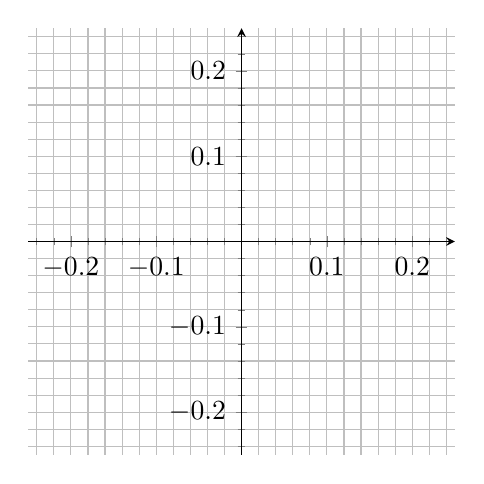
\begin{tikzpicture} 
	\begin{axis}[
		axis x line=middle, axis y line=middle,     		
		%xtick={-5,-4,...,5},
		%ytick={-5,-4,...,5},
		minor x tick num={4},
		minor y tick num={4},
		grid=both,
		xlabel={$$},     
		ylabel={$$},
		xmin=-\xmax.25,xmax=\xmax.25,
		ymin=-\ymax.25,ymax=\ymax.25,     		width=7cm,     		height=7cm] 		
%\addplot[red,very thick,mark=noner,smooth]{x^4-4*x^2}; 
	\end{axis}
\end{tikzpicture}
\end{enumerate}
\end{multicols}

\vfill
\end{document}
